% ---------
% Preamble.
% ---------

% Document type.
\documentclass{article}

% Import custom style.
\usepackage{../.preamble/tikz_diagrams_template}

% Color theme (black, red, blue, green, orange, purple, gold).
\colortheme{blue}

% ---------
% Document.
% ---------

\begin{document}

    % -----------------
    % TikZ environment.
    % -----------------

    \begin{tikzpicture}

        % -----------------
        % Airplane drawing.
        % -----------------
        
        \node[anchor=south west,inner sep=0] (image) at (0,0) {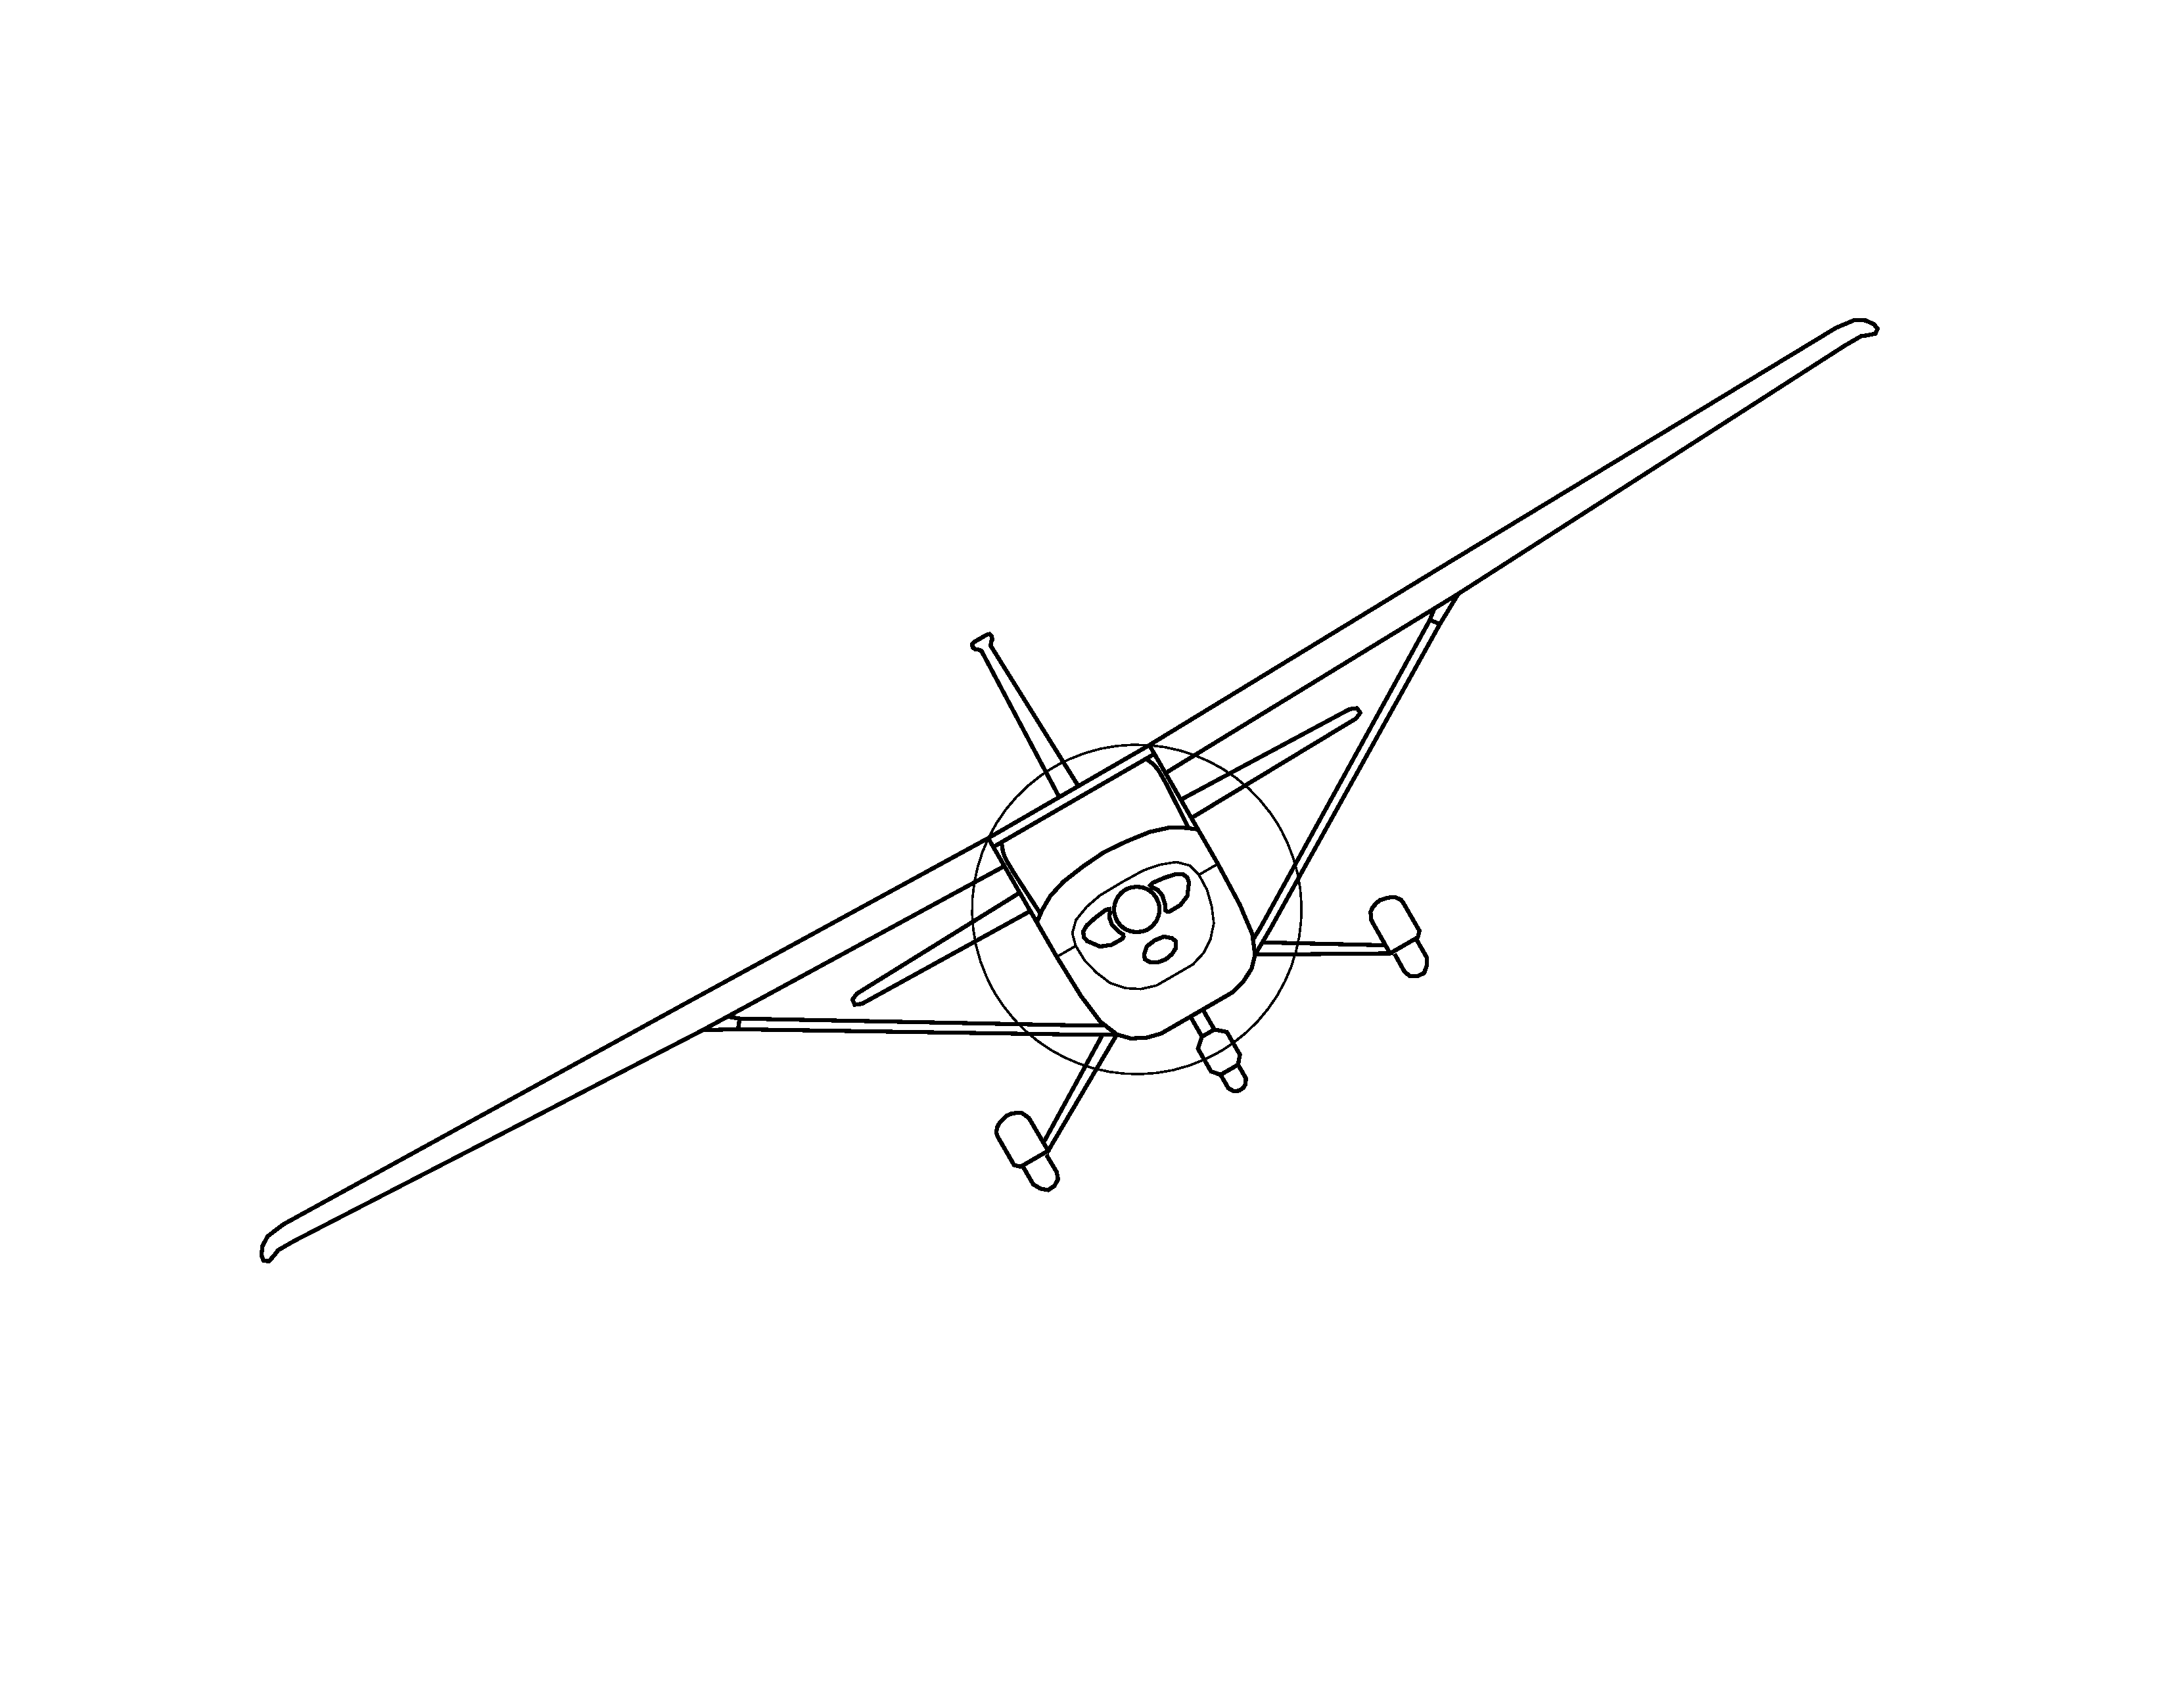
\includegraphics[width=0.6\textwidth]{../.images/airplane_roll.eps}};

        % -----------
        % Parameters.
        % -----------
        
        % Origin.
        \pgfmathsetmacro{\Ox}{5.16}
        \pgfmathsetmacro{\Oy}{3.52}

        % pitch angle [deg]
        \pgfmathsetmacro{\yawangle}{30}
        
        % Axes length.
        \pgfmathsetmacro{\axlen}{4}

        % arc radius
        \pgfmathsetmacro{\arcrad}{0.9*\axlen}

        % -----------
        % Body frame.
        % -----------
        
        % yb-axis endpoint
        \pgfmathsetmacro{\ybx}{\Ox-cos(\yawangle)*\axlen}
        \pgfmathsetmacro{\yby}{\Oy-sin(\yawangle)*\axlen}

        % zb-axis endpoint
        \pgfmathsetmacro{\zbx}{\Ox+sin(\yawangle)*\axlen}
        \pgfmathsetmacro{\zby}{\Oy-cos(\yawangle)*\axlen}

        % Body axes.
        \draw[line width=0.5mm](\Ox,\Oy)--(\ybx,\yby)node[pos=1.08]{$y_{b}$};
        \draw[line width=0.5mm](\Ox,\Oy)--(\zbx,\zby)node[pos=1.06]{$z_{b}$};

        % ------------
        % World frame.
        % ------------
        
        % yw-axis endpoint
        \pgfmathsetmacro{\ywx}{\Ox-\axlen}
        \pgfmathsetmacro{\ywy}{\Oy}

        % zw-axis endpoint
        \pgfmathsetmacro{\zwx}{\Ox}
        \pgfmathsetmacro{\zwy}{\Oy-\axlen}

        % World axes.
        \draw[dotted,line width=0.5mm](\Ox,\Oy)--(\ywx,\ywy)node[pos=1.08]{$y_{w}$};
        \draw[dotted,line width=0.5mm](\Ox,\Oy)--(\zwx,\zwy)node[pos=1.06]{$z_{w}$};

        % -----------
        % Roll angle.
        % -----------

        % arrow 1 starting point
        \pgfmathsetmacro{\arcxa}{\Ox-\arcrad}
        \pgfmathsetmacro{\arcya}{\Oy}

        % arrow 1
        \draw[-mylatex',color_theme,thick](\arcxa,\arcya)arc(180:210:\arcrad)node[midway,left,yshift=5]{$\phi_{\mathrm{world}\to\mathrm{body}}$};

        % arrow 2 starting point
        \pgfmathsetmacro{\arcxb}{\Ox}
        \pgfmathsetmacro{\arcyb}{\Oy-\arcrad}

        % arrow 2
        \draw[-mylatex',color_theme,thick](\arcxb,\arcyb)arc(-90:-60:\arcrad)node[midway,below,yshift=-4,xshift=4]{$\phi_{\mathrm{world}\to\mathrm{body}}$};
        
    \end{tikzpicture}

\end{document}